\appendix

\chapter{Appendix}\label{sec:appendix}

\begin{xltabular}{\textwidth}{lX}
        \toprule
        \textbf{Parameter}                  & \textbf{Description} \\
        \midrule
        \texttt{RDC\_gamma}                 & The discount factor ($\gamma$) that determines the present value of future rewards, balancing immediate and long-term gains in the Bellman equation. \\
        \texttt{RDC\_tau}                   & The interpolation factor ($\tau$) for the soft update of the target network, controlling how quickly the target network tracks the policy network. \\
        \midrule
        \texttt{RDC\_state\_dim}            & The dimensionality of the input state vector, determined by the number of geographic zones and the features used to describe each zone. \\
        \texttt{RDC\_hidden\_size}          & The number of neurons in each hidden layer of the Multi-Head Deep Q-Network, defining the model's learning capacity. \\
        \midrule
        \texttt{RDC\_lr}                    & The initial learning rate ($\alpha_{lr}$) for the Adam optimizer, controlling the step size of gradient descent updates. \\
        \texttt{RDC\_lr\_step\_size}        & The number of training steps after which the learning rate is multiplicatively decayed. \\
        \texttt{RDC\_lr\_gamma}             & The multiplicative factor ($\gamma_{lr}$) by which the learning rate is decayed. \\
        \midrule
        \texttt{RDC\_rb\_capacity}          & The maximum number of transition experiences stored in the replay buffer. \\
        \texttt{RDC\_batch\_size}           & The number of experiences sampled from the replay buffer for each training step. \\
        \texttt{RDC\_per\_alpha}            & The prioritization exponent ($\alpha_{PER}$), controlling how aggressively priorities are used for sampling (0 = uniform sampling, 1 = full prioritization). \\
        \texttt{RDC\_per\_beta\_start}      & The initial value of the importance-sampling exponent ($\beta_{PER}$), which is annealed to 1.0 to correct for the bias introduced by prioritized sampling. \\
        \texttt{RDC\_per\_beta\_frames}     & The number of training frames over which the \gls{per} exponent $\beta$ is annealed to 1.0. \\
        \midrule
        \texttt{RDC\_epsilon\_start}        & The initial probability ($\epsilon_{start}$) of selecting a random action to encourage exploration. \\
        \texttt{RDC\_epsilon\_end}          & The minimum final probability ($\epsilon_{min}$) of selecting a random action, ensuring some exploration persists. \\
        \texttt{RDC\_epsilon\_decay}        & The multiplicative factor ($\delta_{\epsilon}$) used to gradually decrease the exploration rate from its initial value to its final value. \\
        \midrule
        \texttt{RDC\_weight\_demand}        & The weighting coefficient for the satisfied demand component ($w_{demand}^{RDC}$) in the composite reward function. \\
        \texttt{RDC\_weight\_cost}          & The weighting coefficient for the rebalancing cost penalty component ($w_{cost}^{RDC}$) in the composite reward function. \\
        \texttt{RDC\_weight\_gini}          & The weighting coefficient for the Gini index component ($w_{gini}^{RDC}$) in the composite reward function. \\
        \bottomrule
    \caption{Configurable Hyperparameters for the Regional Distribution Coordinator (RDC) Agent. This table lists and describes the complete set of 17 hyperparameters that define the behavior and architecture of the RDC agent. These parameters govern aspects of the learning algorithm, network architecture, prioritized experience replay buffer, exploration strategy, and reward weights. The systematic optimization of these hyperparameters, except the reward weights, was crucial for achieving peak performance and is detailed in \autoref{sec:evaluation-ho-rdc}.}
    \label{tab:rdc_hyperparameters_detailed}
\end{xltabular}

\begin{xltabular}{\textwidth}{lX}
        \toprule
        Parameter & Description \\
        \midrule
        \texttt{UIC\_lr}                & The learning rate for the Adam optimizer, which controls the step size of the gradient-based updates to the policy and value function networks. \\
        \texttt{UIC\_n\_steps}          & The number of simulation steps collected from the environment during each rollout phase before a policy update is performed. \\
        \texttt{UIC\_batch\_size}       & The number of training samples used in one minibatch for a single gradient descent step. \\
        \texttt{UIC\_clip\_range}       & The clipping parameter for PPO's surrogate objective function. It defines a small, acceptable range for the policy ratio, preventing excessively large policy updates and ensuring training stability. \\
        \texttt{UIC\_ent\_coeff}        & The coefficient for the entropy bonus term in the loss function. A positive coefficient encourages exploration by penalizing policies that become too deterministic. \\
        \texttt{UIC\_vf\_coeff}         & The coefficient for the value function loss term in the total loss calculation. It balances the updates between the policy (actor) and the value function (critic). \\
        \midrule
        \texttt{UIC\_gamma}             & The discount factor applied to future rewards. It determines the present value of future rewards, influencing how far-sighted the agent's planning horizon is. \\
        \texttt{UIC\_gae\_lambda}       & The lambda parameter for Generalized Advantage Estimation (GAE). It provides a trade-off between bias (low lambda) and variance (high lambda) in the advantage function estimates. \\
        \texttt{UIC\_target\_kl}        & If the \glsfirst{kl} divergence between the new and old policies exceeds this target, updates for the current iteration are stopped. \\
        \midrule
        \texttt{UIC\_num\_layers}       & The number of hidden layers used in the neural network architecture for both the policy (actor) and value (critic) networks. \\
        \texttt{UIC\_hidden\_size}      & The number of neurons within each hidden layer of the policy and value networks. \\
        \texttt{UIC\_activation\_fn}    & The non-linear activation function applied to the output of neurons in the hidden layers. \\
        \midrule
        \texttt{UIC\_weight\_demand}    & The weighting coefficient for the satisfied demand component ($w_{demand}^{UIC}$) in the composite reward function. \\
        \texttt{UIC\_weight\_cost}      & The weighting coefficient for the rebalancing cost penalty component ($w_{cost}^{UIC}$) in the composite reward function. \\
        \texttt{UIC\_weight\_gini}      & The weighting coefficient for the Gini index component ($w_{gini}^{UIC}$) in the composite reward function. \\
        \bottomrule
    \caption{Configurable Hyperparameters for the User-Incentive Coordinator (UIC) Agent. This table presents the 15 configurable hyperparameters for the PPO-based UIC agent. The parameters control the core PPO algorithm, network architecture, stability mechanisms, and reward weights. These values, except the reward weights, were systematically tuned to optimize the agent's ability to learn an effective local incentive policy (see \autoref{sec:evaluation-ho-uic}).}
    \label{tab:uic_hyperparameters_detailed}
\end{xltabular}


\begin{table}[!htb]
    \centering
    \begin{tabular}{lll}
        \toprule
        \textbf{Parameter} & \textbf{Range} & \textbf{Step} \\
        \midrule
        \texttt{RDC\_lr}                 & $[1e^{-6}, 1e^{-4}]$      & log-uniform \\
        \texttt{RDC\_lr\_step\_size}     & [500, 5000]               & 250 \\
        \texttt{RDC\_lr\_gamma}          & [0.5, 0.99]              & 0.01 \\
        \texttt{RDC\_gamma}              & [0.90, 0.99]              & 0.001\\
        \midrule
        \texttt{RDC\_hidden\_size}       & \{64, 128, 256, 512\}     & - \\
        \texttt{RDC\_batch\_size}        & \{64, 128, 256, 512\}     & - \\
        \texttt{RDC\_tau}                & [0.0001, 0.1]            & 0.0001 \\
        \midrule
        \texttt{RDC\_rb\_capacity}       & [5000, 120000]             & log-uniform \\
        \texttt{RDC\_per\_alpha}         & [0.0, 1.0]                & 0.1\\
        \texttt{RDC\_per\_beta\_start}   & [0.1, 0.6]                & 0.1\\
        \texttt{RDC\_per\_beta\_frames}  & [3000, 50000]           & log-uniform\\
        \midrule
        \texttt{RDC\_epsilon\_start}     & 1.0                       & - \\
        \texttt{RDC\_epsilon\_end}       & [0.01, 0.20]              & 0.01 \\
        \texttt{RDC\_epsilon\_decay}     & [0.95, 0.9999]            & log-uniform\\
        \midrule
    \end{tabular}
    \caption{RDC Hyperparameter Optimization Search Space (Round 1). This table defines the broad search spaces for all 14 RDC hyperparameters used in the initial, exploratory round of the coarse-to-fine optimization process. This first round was designed to identify promising regions within a wide range of possible values for each parameter group.}
    \label{tab:rdc_ho_first_round}
\end{table}

\begin{table}[!htb]
    \centering
    \begin{tabular}{lll}
        \toprule
        \textbf{Parameter} & \textbf{Range} & \textbf{Step} \\
        \midrule
        \texttt{RDC\_lr}                 & $[1e^{-6}, 1e^{-5}]$      & log-uniform \\
        \texttt{RDC\_lr\_step\_size}     & [2000, 5000]               & 250 \\
        \texttt{RDC\_lr\_gamma}          & [0.88, 0.99]              & 0.01 \\
        \texttt{RDC\_gamma}              & [0.900, 0.999]              & 0.001\\
        \midrule
        \texttt{RDC\_hidden\_size}       & \{128, 256, 512\}     & - \\
        \texttt{RDC\_batch\_size}        & \{128, 256, 512\}     & - \\
        \texttt{RDC\_tau}                & [0.003, 0.010]            & 0.001 \\
        \midrule
        \texttt{RDC\_rb\_capacity}       & [1000, 45000]             & 1,000\\
        \texttt{RDC\_per\_alpha}         & [0.0, 0.8]                & 0.1\\
        \texttt{RDC\_per\_beta\_start}   & [0.1, 0.55]                & 0.1\\
        \texttt{RDC\_per\_beta\_frames}  & [1000, 50000]           & 10000\\
        \midrule
        \texttt{RDC\_epsilon\_start}     & 1.0                       & - \\
        \texttt{RDC\_epsilon\_end}       & [0.01, 0.18]              & 0.01 \\
        \texttt{RDC\_epsilon\_decay}     & [0.950, 0.999]            & 0.001\\
        \midrule
    \end{tabular}
    \caption{RDC Hyperparameter Optimization Search Space (Round 2). This table details the refined search spaces for the second round of the RDC hyperparameter optimization. The ranges were narrowed or shifted based on the results of the first round to focus the search on the most promising areas of the parameter space.}
    \label{tab:rdc_ho_second_round}
\end{table}
\begin{table}[!htb]
    \centering
    \begin{tabular}{lll}
        \toprule
        \textbf{Parameter} & \textbf{Range} & \textbf{Step} \\
        \midrule
        \texttt{RDC\_lr}                 & $[1e^{-6}, 1e^{-5}]$      & log-uniform \\
        \texttt{RDC\_lr\_step\_size}     & [1000, 6000]               & 100 \\
        \texttt{RDC\_lr\_gamma}          & [0.7, 0.8]              & 0.001 \\
        \texttt{RDC\_gamma}              & [0.96, 0.99]              & 0.001\\
        \midrule
        \texttt{RDC\_hidden\_size}       & \{256, 512, 1024\}                 & - \\
        \texttt{RDC\_batch\_size}        & \{256, 512, 1024\}          & - \\
        \texttt{RDC\_tau}                & [0.0078, 0.0102]           & 0.0001 \\
        \midrule
        \texttt{RDC\_rb\_capacity}       & [5000, 70000]             & log-uniform\\
        \texttt{RDC\_per\_alpha}         & [0.2, 1.0]              & 0.1\\
        \texttt{RDC\_per\_beta\_start}   & [0.25, 0.56]              & 0.01\\
        \texttt{RDC\_per\_beta\_frames}  & [5000, 65000]           & log-uniform\\
        \midrule
        \texttt{RDC\_epsilon\_start}     & 1.0                       & - \\
        \texttt{RDC\_epsilon\_end}       & [0.06, 0.075]              & 0.001 \\
        \texttt{RDC\_epsilon\_decay}     & [0.96, 0.975]            & 0.001\\
        \midrule
    \end{tabular}
    \caption{RDC Hyperparameter Optimization Search Space (Round 3). This table lists the final search spaces for the third and final round of the RDC hyperparameter optimization, where all 14 parameters were tuned simultaneously. These tightly constrained ranges reflect the knowledge gained from the previous two rounds and were used to fine-tune the agent's configuration.}
    \label{tab:rdc_ho_final_round}
\end{table}


\begin{table}[!htb]
    \centering
    \begin{tabular}{lll}
        \toprule
        \textbf{Parameter} & \textbf{Range} & \textbf{Step} \\
        \midrule
        \texttt{UIC\_lr}                 & $[5e^{-6}, 5e^{-4}]$      & log-uniform \\
        \texttt{UIC\_n\_steps}     & \{256, 512, 1024, 2048\}              & - \\
        \texttt{UIC\_batch\_size}     & \{32, 64, 128, 256\}              & - \\
        \texttt{UIC\_clip\_range}     & [0.1, 0.3]              & 0.05 \\
        \texttt{UIC\_ent\_coeff}     & $[1e^{-5}, 1e^{-3}]$              & log-uniform \\
        \texttt{UIC\_vf\_coeff}     & [0.4, 0.8]              & 0.05 \\
        \midrule
        \texttt{UIC\_hidden\_size}       & \{64, 96, 128, 256\}     & - \\
        \texttt{UIC\_n\_layers}        & \{2, 3, 4\}     & - \\
        \texttt{UIC\_activation\_fn}                & \{ReLU, TanH, LeakyReLU, SiLU\}            & - \\
        \midrule
        \texttt{UIC\_gamma}       & [0.95, 0.999]             & log-uniform\\
        \texttt{UIC\_gae\_lambda}         & [0.90, 0.98]                & 0.01\\
        \texttt{UIC\_target\_kl}   & \{None, 0.01, 0.015, 0.02, 0.025\}                & -\\
        \bottomrule
    \end{tabular}
    \caption{UIC Hyperparameter Optimization Search Space (Round 1). This table specifies the initial, broad search spaces for the hyperparameters of the UIC agent in the first round of optimization. This round aimed to explore a wide variety of configurations to identify potentially effective parameter settings for the PPO algorithm.}
    \label{tab:uic_ho_first_round}
\end{table}

\begin{table}[!htb]
    \centering
    \begin{tabular}{lll}
        \toprule
        \textbf{Parameter} & \textbf{Range} & \textbf{Step} \\
        \midrule
        \texttt{UIC\_lr}                & $[1e^{-5}, 1e^{-4}]$      & log-uniform \\
        \texttt{UIC\_n\_steps}          & \{256, 512, 768\}         & - \\
        \texttt{UIC\_batch\_size}       & \{32, 64, 128\}           & - \\
        \texttt{UIC\_clip\_range}       & [0.5, 0.3]                & 0.05 \\
        \texttt{UIC\_ent\_coeff}        & $[1e^{-5}, 1e^{-4}]$      & log-uniform \\
        \texttt{UIC\_vf\_coeff}         & [0.65, 0.85]              & 0.05 \\
        \midrule
        \texttt{UIC\_hidden\_size}      & \{96, 128, 256\}          & - \\
        \texttt{UIC\_n\_layers}         & \{2, 3\}                  & - \\
        \texttt{UIC\_activation\_fn}    & \{ReLU, TanH, LeakyReLU\} & - \\
        \midrule
        \texttt{UIC\_gamma}             & [0.95, 0.99]              & log-uniform \\
        \texttt{UIC\_gae\_lambda}       & [0.90, 0.97]              & 0.01\\
        \texttt{UIC\_target\_kl}        & \{0.01, 0.015, 0.02\}     & -\\
        \bottomrule
    \end{tabular}
    \caption{UIC Hyperparameter Optimization Search Space (Round 2). This table outlines the narrowed and refined search spaces used in the second round of the UIC's hyperparameter optimization. Based on the initial results, the search was concentrated on more promising value ranges for each parameter group.}
    \label{tab:uic_ho_second_round}
\end{table}

\begin{table}[!htb]
    \centering
    \begin{tabular}{lll}
        \toprule
        \textbf{Parameter} & \textbf{Range} & \textbf{Step} \\
        \midrule
        \texttt{UIC\_lr}                & $[2e^{-5}, 6e^{-5}]$      & log-uniform \\
        \texttt{UIC\_n\_steps}          & \{256, 512\}              & - \\
        \texttt{UIC\_batch\_size}       & \{32, 64\}                & - \\
        \texttt{UIC\_clip\_range}       & [0.25, 0.3]               & 0.01 \\
        \texttt{UIC\_ent\_coeff}        & $[2e^{-5}, 1e^{-4}]$      & log-uniform \\
        \texttt{UIC\_vf\_coeff}         & [0.65, 0.75]              & 0.01 \\
        \midrule
        \texttt{UIC\_hidden\_size}      & \{128, 256\}              & - \\
        \texttt{UIC\_n\_layers}         & \{2\}                     & - \\
        \texttt{UIC\_activation\_fn}    & \{ReLU, LeakyReLU\}       & - \\
        \midrule
        \texttt{UIC\_gamma}             & [0.95, 0.98]              & log-uniform \\
        \texttt{UIC\_gae\_lambda}       & [0.94, 0.97]              & 0.01\\
        \texttt{UIC\_target\_kl}        & \{0.02\}                  & -\\
        \bottomrule
    \end{tabular}
    \caption{UIC Hyperparameter Optimization Search Space (Round 3). This table defines the search spaces for the final, unified optimization round for the UIC agent. These focused ranges were used to perform a fine-tuning sweep across all 15 hyperparameters simultaneously to arrive at the final optimal configuration.}
    \label{tab:uic_ho_final_round}
\end{table}

\begin{figure}
    \centering
    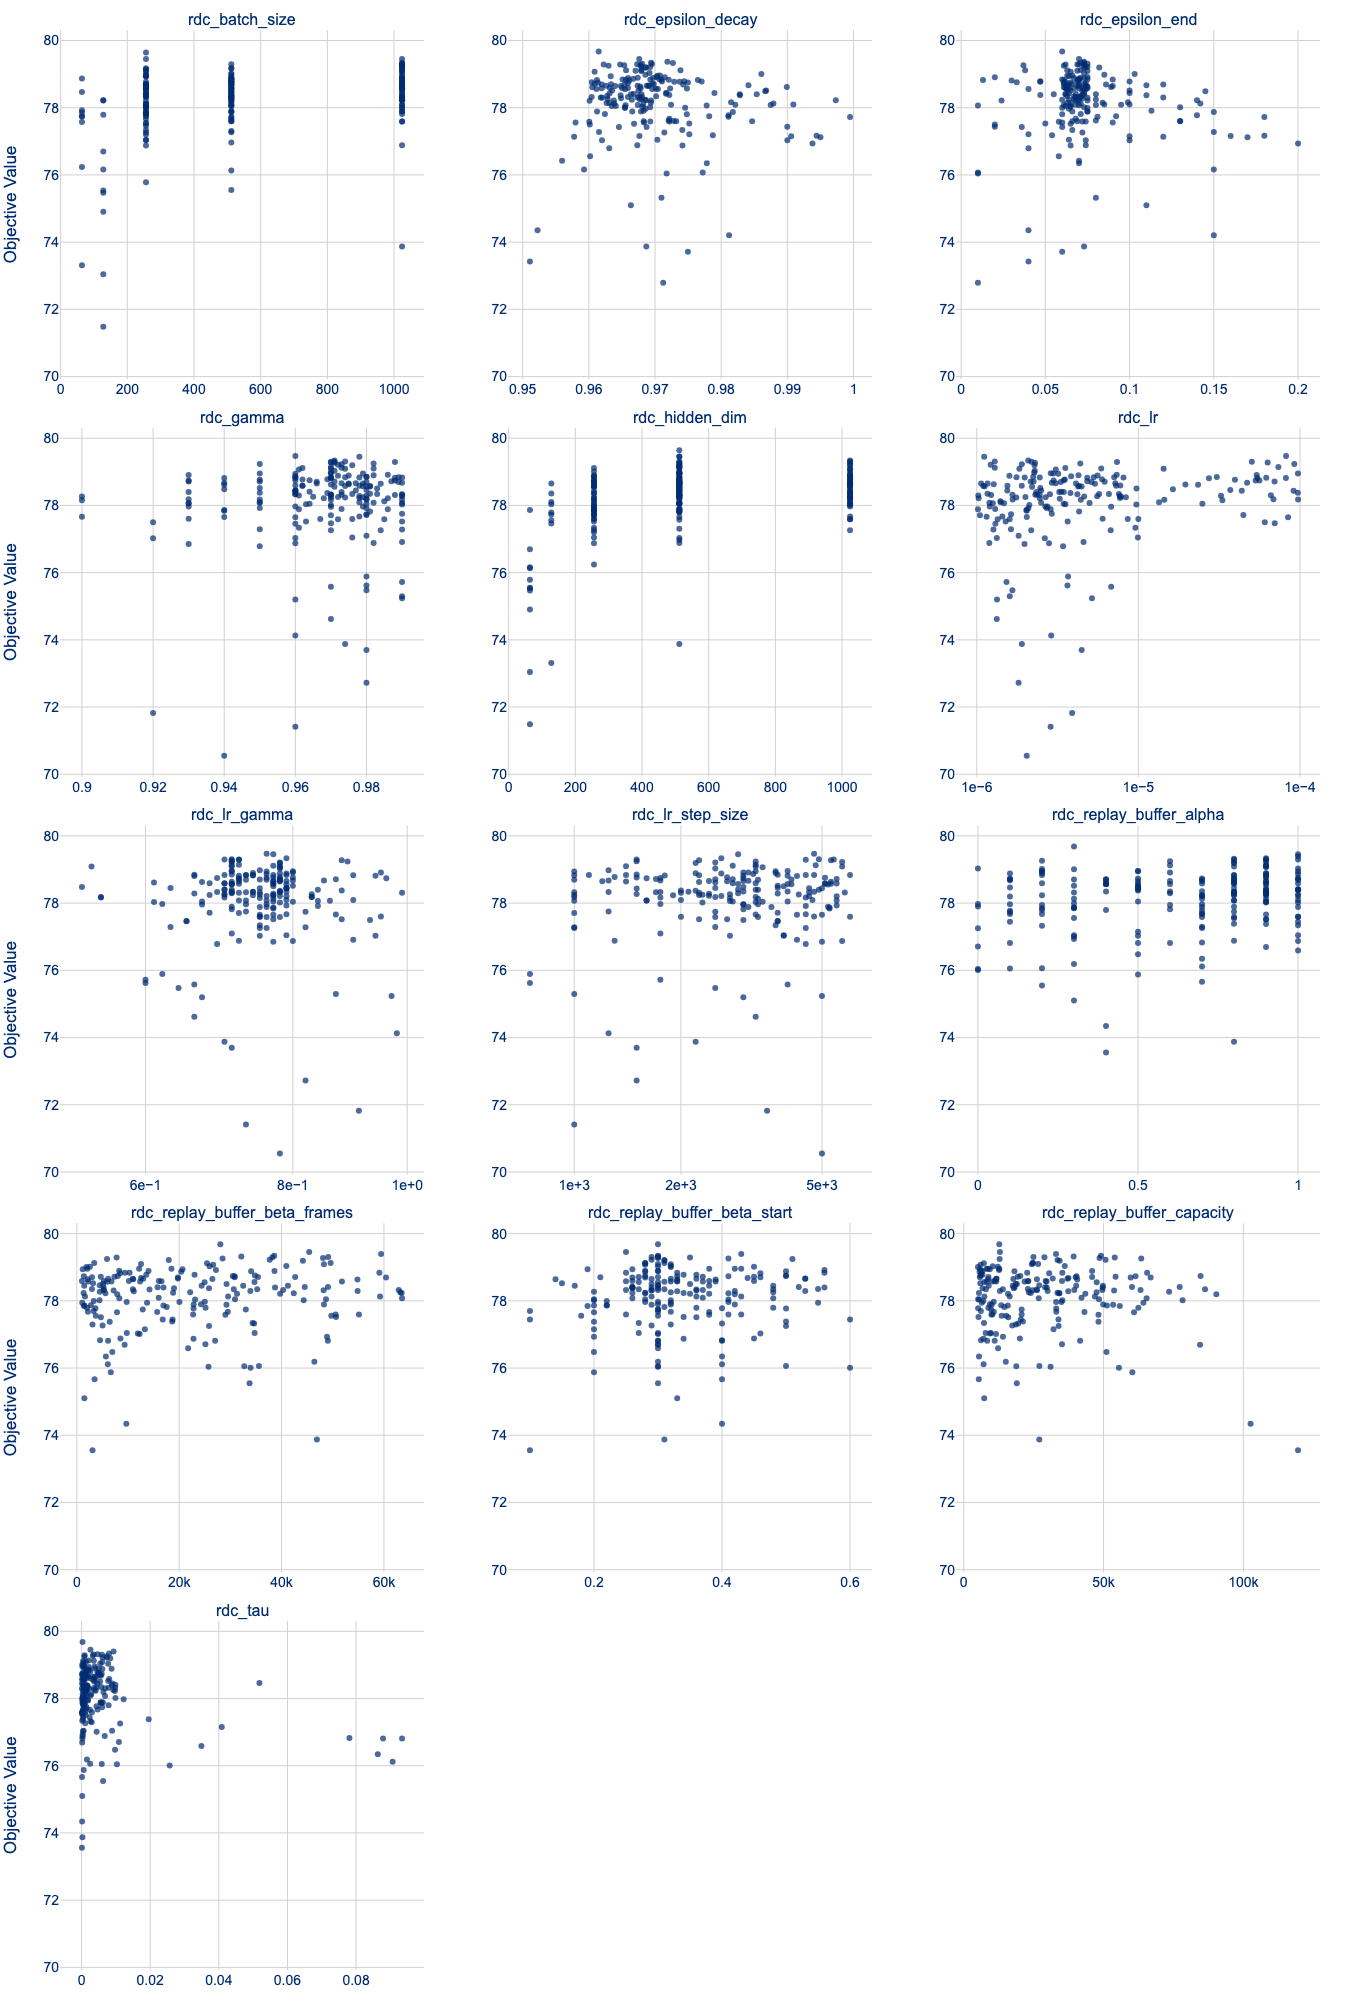
\includegraphics[width=.9\linewidth]{content/figures/RDC_full_slice_plot.png}
    \caption{Full Slice Plot for All RDC Hyperparameter Optimization Trials. This figure provides the complete set of slice plots for all 14 hyperparameters optimized for the Regional Distribution Coordinator (RDC) agent. Each subplot displays the objective value (y-axis) achieved across the range of values tested for a single hyperparameter (x-axis) over the 500 trials. This comprehensive visualization allows for a detailed inspection of the sensitivity and optimal ranges for every parameter governing the MH-DQN agent's performance.}
    \label{fig:rdc-full-slice-plot}
\end{figure}

\begin{figure}
    \centering
    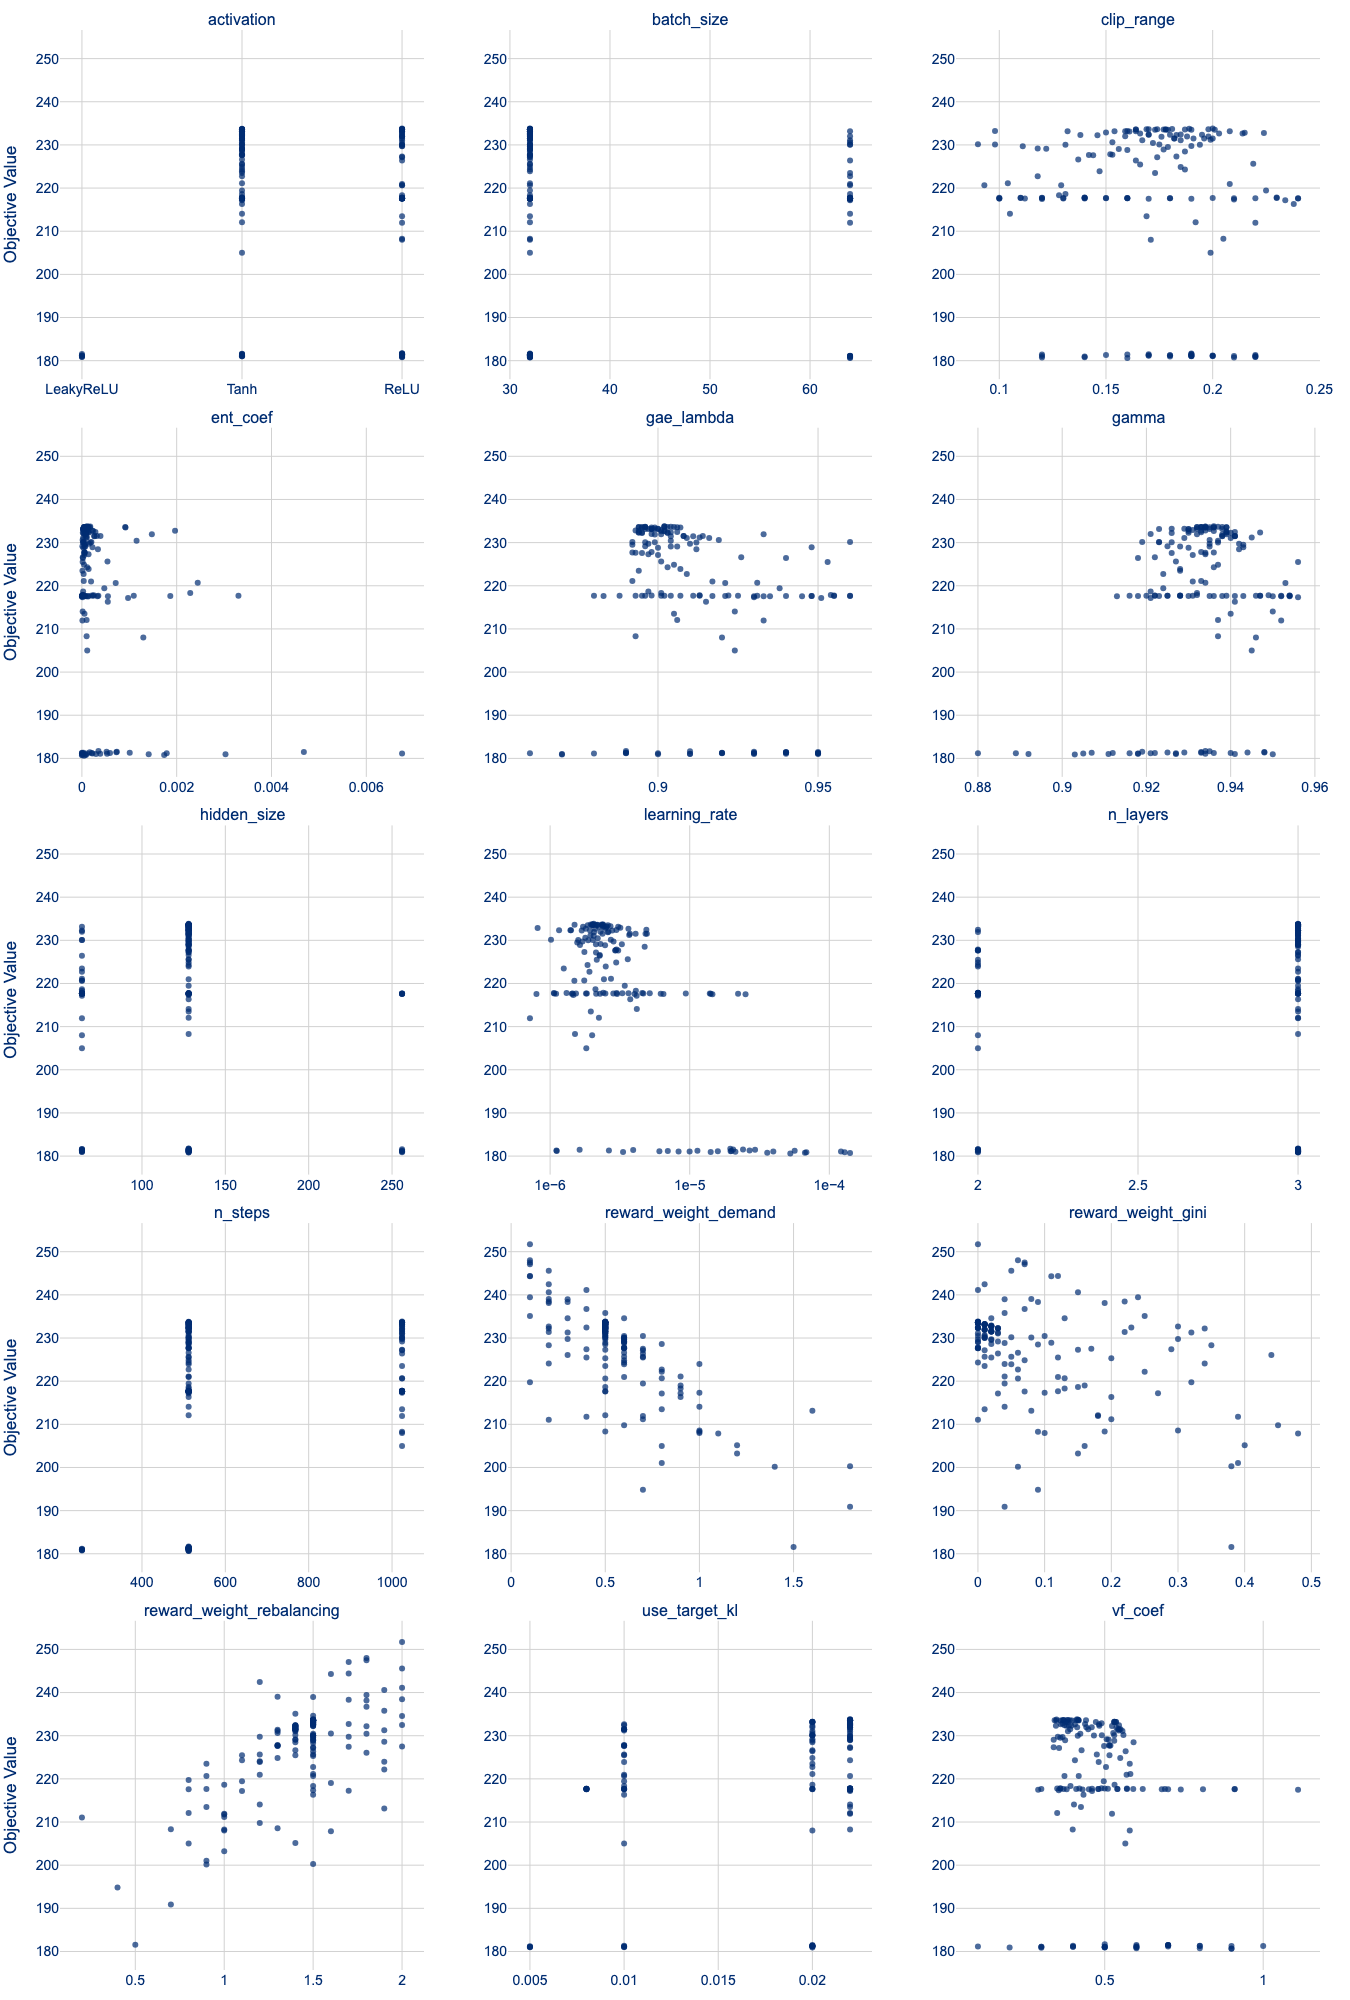
\includegraphics[width=\linewidth]{content/figures/UIC_full_slice_plot.png}
    \caption{ Full Slice Plot for All UIC Hyperparameter Optimization Trials. This figure presents the complete collection of slice plots for all 12 hyperparameters that were tuned for the User-Incentive Coordinator (UIC) agent. Each subplot illustrates how the final objective value (y-axis) varied with the value of a specific hyperparameter (x-axis) during the optimization process. This detailed view is useful for understanding the complex interplay between the PPO algorithm's parameters and its resulting performance.}
    \label{fig:uic-full-slice-plot}
\end{figure}